\documentclass[12pt, twoside]{article}
\usepackage[letterpaper, margin=1in, headsep=0.5in]{geometry}
\usepackage[english]{babel}
\usepackage[utf8]{inputenc}
\usepackage{amsmath}
\usepackage{amsfonts}
\usepackage{amssymb}
\usepackage{tikz}
\usetikzlibrary{quotes, angles}
\usepackage{graphicx}
%\usepackage{pgfplots}
%\pgfplotsset{width=10cm,compat=1.9}
%\usepgfplotslibrary{statistics}
%\usepackage{pgfplotstable}
%\usepackage{tkz-fct}
%\usepackage{venndiagram}
\usepackage{enumitem}
\usepackage{multicol}


\usepackage{fancyhdr}
\pagestyle{fancy}
\fancyhf{}
\fancyhead[LE]{\thepage}
\fancyhead[RO]{\thepage \\Name: \hspace{4cm} \,\\}
\fancyhead[LO]{BECA / Dr. Huson / Geometry 10th Grade\\* Unit 9: Congruence transformations \\ 6 March 2020}

\renewcommand{\headrulewidth}{0pt}

\begin{document}
\subsubsection*{9.9b Quiz: Rigid motions, translation, reflection, rotation (No Calculator)}
  \begin{enumerate}

  \item State the translation that would map $M(-2,9)$ onto $M'(-1,8)$. \vspace{2cm}
  
  \item On the set of axes below, $\triangle ABC \cong \triangle STU$. \\[0.5cm]
  Describe the rigid motion that maps $\triangle ABC$ onto $\triangle STU$.
  \begin{flushright}
      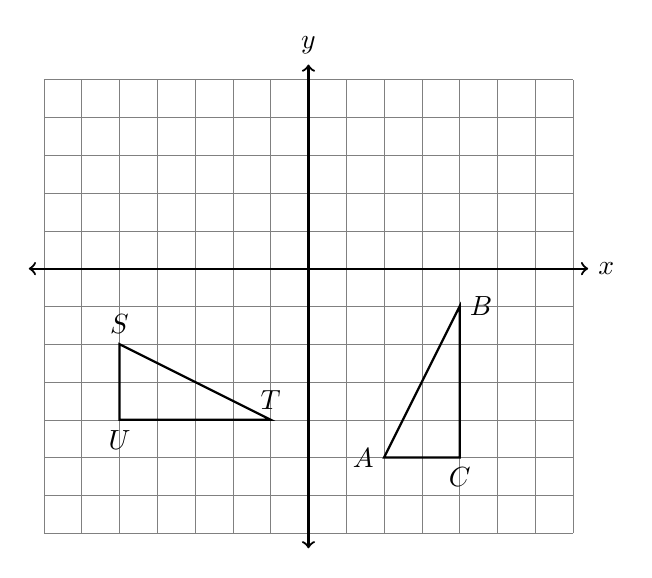
\begin{tikzpicture}[scale=.48]
      \draw [help lines] (-7,-7) grid (7,5);
      \draw [thick, <->] (-7.4,0) -- (7.4,0) node [right] {$x$};
      \draw [thick, <->] (0,-7.4)--(0,5.4) node [above] {$y$};  
      \draw [thick]
        (2,-5) node[left] {$A$}--
        (4,-1) node[right] {$B$}--
        (4,-5) node[below] {$C$}--cycle;
      \draw [thick]
      (-5,-2) node[above] {$S$}--
      (-1,-4) node[above] {$T$}--
      (-5,-4) node[below] {$U$}--cycle;
    \end{tikzpicture}
  \end{flushright}

  \item Rotate $\triangle JKL$ $90^\circ$ clockwise around the origin on the axes below, labeling the image $\triangle J'K'L'$.
  \begin{center}
      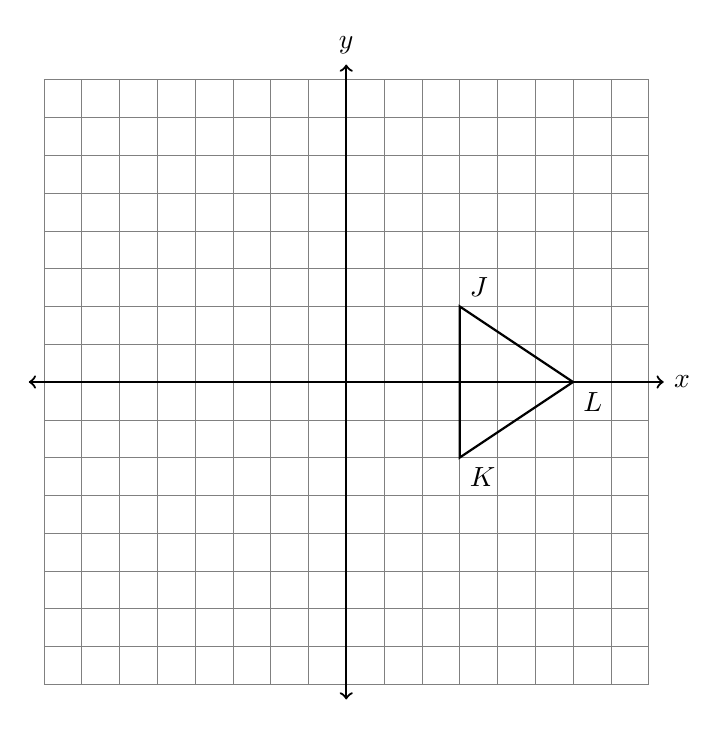
\begin{tikzpicture}[scale=.48]
      \draw [help lines] (-8,-8) grid (8,8);
      \draw [thick, <->] (-8.4,0) -- (8.4,0) node [right] {$x$};
      \draw [thick, <->] (0,-8.4)--(0,8.4) node [above] {$y$};  
      \draw [thick]
        (3,2) node[above right] {$J$}--
        (3,-2) node[below right] {$K$}--
        (6,0) node[below right] {$L$}--cycle;  
    \end{tikzpicture}
  \end{center}
  
  \begin{multicols}{2}
    [\item The quadrilateral $MATH$ is mapped to $M'A'T'H'$ by a rigid motion. What transformation a been applied?]  \vspace{0.5cm}
    \begin{enumerate}
      \item Dilation
      \item Reflection
      \item Rotation
      \item Translation
    \end{enumerate}
    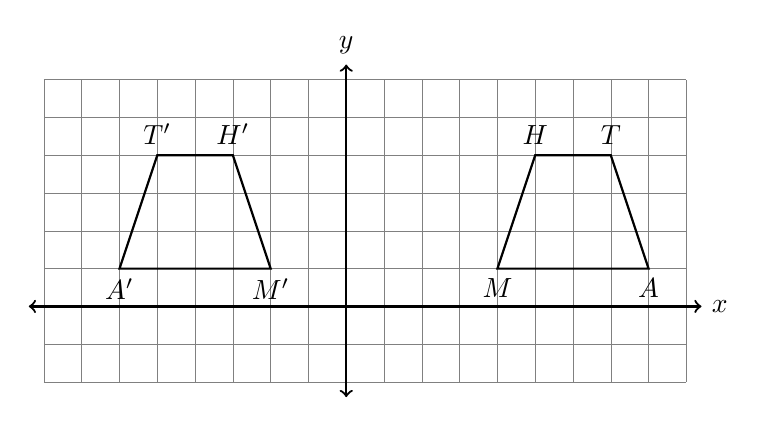
\begin{tikzpicture}[scale=.48]
      \draw [help lines] (-8,-2) grid (9,6);
      \draw [thick, <->] (-8.4,0) -- (9.4,0) node [right] {$x$};
      \draw [thick, <->] (0,-2.4)--(0,6.4) node [above] {$y$};  
      \draw [thick]
        (4,1) node[below] {$M$}--
        (8,1) node[below] {$A$}--
        (7,4) node[above] {$T$}--
        (5,4) node[above] {$H$}--cycle;
      \draw [thick]
        (-2,1) node[below] {$M'$}--
        (-6,1) node[below] {$A'$}--
        (-5,4) node[above] {$T'$}--
        (-3,4) node[above] {$H'$}--cycle; 
    \end{tikzpicture}
  \end{multicols}

  \item Determine and state the sequence of transfromations applied to map $BECA$ to $B''E''C''A''$.
  \begin{flushright}
      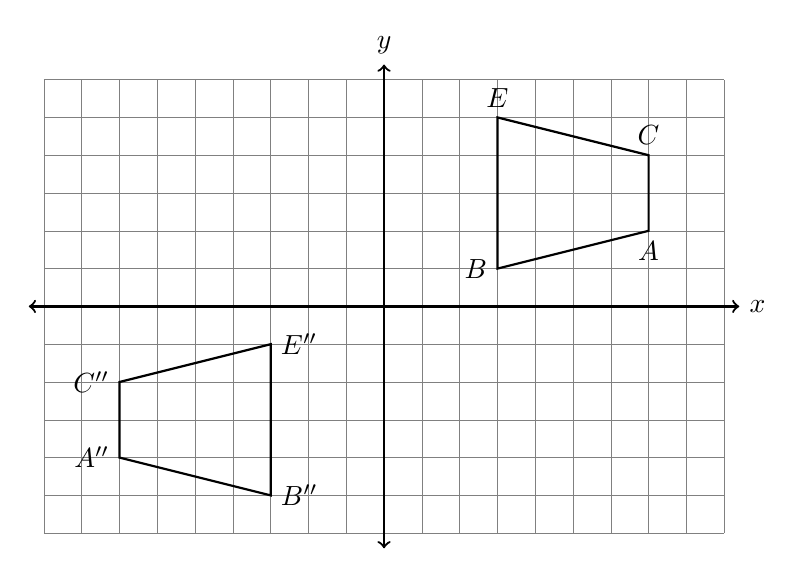
\begin{tikzpicture}[scale=.48]
      \draw [help lines] (-9,-6) grid (9,6);
      \draw [thick, <->] (-9.4,0) -- (9.4,0) node [right] {$x$};
      \draw [thick, <->] (0,-6.4)--(0,6.4) node [above] {$y$};  
      \draw [thick]
        (3,1) node[left] {$B$}--
        (3,5) node[above] {$E$}--
        (7,4) node[above] {$C$}--
        (7,2) node[below] {$A$}--cycle;
      \draw [thick]
        (-3,-1) node[right] {$E''$}--
        (-3,-5) node[right] {$B''$}--
        (-7,-4) node[left] {$A''$}--
        (-7,-2) node[left] {$C''$}--cycle; 
    \end{tikzpicture}
  \end{flushright}
 
  \begin{multicols}{2}
    [\item Which of the following would map $\triangle DOG \rightarrow \triangle D'O'G'$?]  \vspace{0.5cm}
    \begin{itemize}
      \item[T \quad F \quad] Reflected across the $y$-axis
      \item[T \quad F \quad] Translated six to the left, down zero
      \item[T \quad F \quad] Slid to the left four, then reflected across the $y$-axis
      \item[T \quad F \quad] $(x,y) \rightarrow (x-6, y+0)$
      \item[T \quad F \quad] Rotated $90^\circ$ clockwise around $(2,0)$
      \item[T \quad F \quad] Reflected across the line $x=2$
    \end{itemize}
    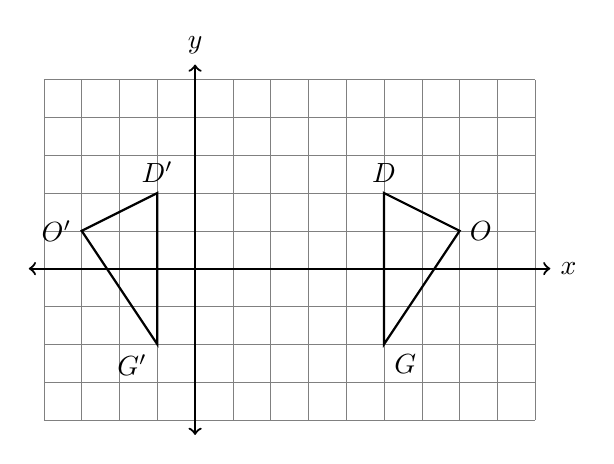
\begin{tikzpicture}[scale=.48]
      \draw [help lines] (-7,-4) grid (6,5);
      \draw [thick, <->] (-7.4,0) -- (6.4,0) node [right] {$x$};
      \draw [thick, <->] (-3,-4.4)--(-3,5.4) node [above] {$y$};  
      \draw [thick]
      (2,2) node[above] {$D$}--
      (4,1) node[right] {$O$}--
      (2,-2) node[below right] {$G$}--cycle;
      \draw [thick]
      (-4,2) node[above] {$D'$}--
      (-6,1) node[left] {$O'$}--
      (-4,-2) node[below left] {$G'$}--cycle;
    \end{tikzpicture}
  \end{multicols}

\newpage
  \item First reflect the trapezoid $BECA$ across the $y$-axis, then move it down 5 and left 1. Label the images $B'E'C'A'$ and $B''E''C''A''$.
    \begin{center}
        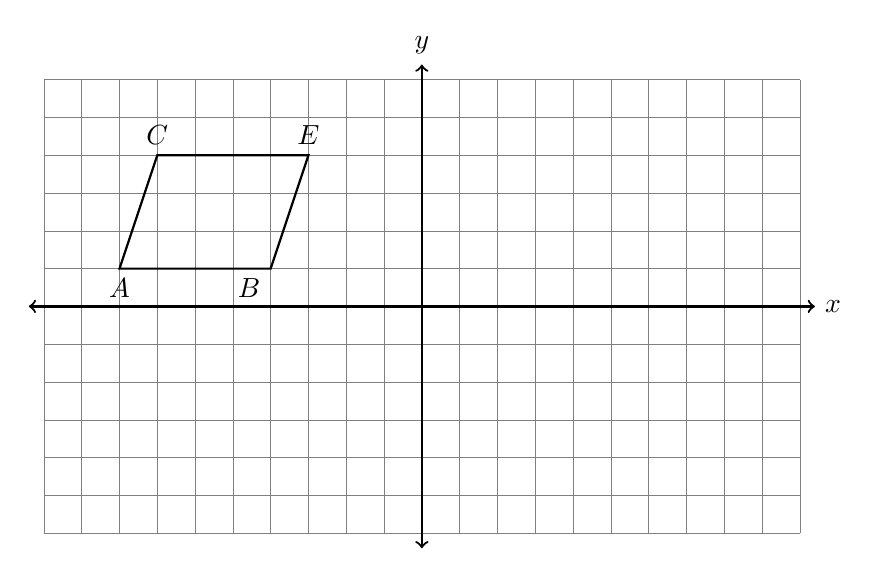
\begin{tikzpicture}[scale=.48]
        \draw [help lines] (-10,-6) grid (10,6);
        \draw [thick, <->] (-10.4,0) -- (10.4,0) node [right] {$x$};
        \draw [thick, <->] (0,-6.4)--(0,6.4) node [above] {$y$};  
        \draw [thick]
          (-4,1) node[below left] {$B$}--
          (-3,4) node[above] {$E$}--
          (-7,4) node[above] {$C$}--
          (-8,1) node[below] {$A$}--cycle;  
      \end{tikzpicture}
    \end{center}


  \item The quadrilateral $ROCK$ undergoes rigid motions, shown below. Describe the sequence of transformations applied.
  \begin{flushright}
      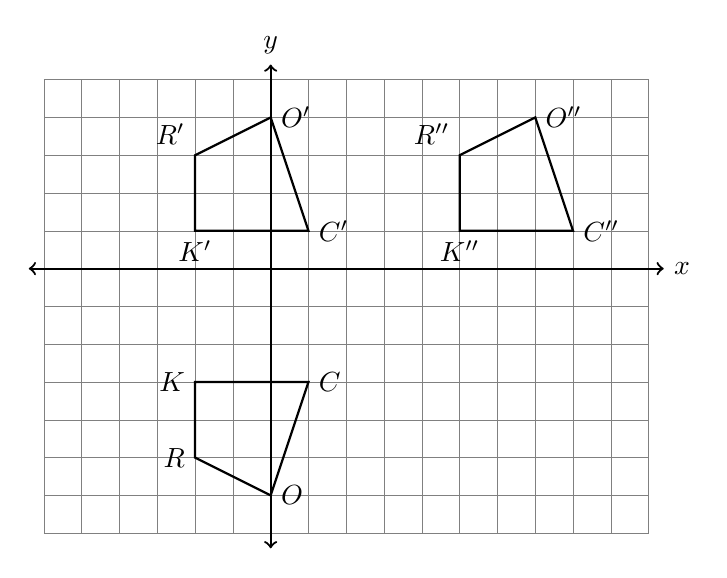
\begin{tikzpicture}[scale=.48]
      \draw [help lines] (-6,-7) grid (10,5);
      \draw [thick, <->] (-6.4,0) -- (10.4,0) node [right] {$x$};
      \draw [thick, <->] (0,-7.4)--(0,5.4) node [above] {$y$};  
      \draw [thick]
        (5,1) node[below] {$K''$}--
        (5,3) node[above left] {$R''$}--
        (7,4) node[right] {$O''$}--
        (8,1) node[right] {$C''$}--cycle;
      \draw [thick]
        (-2,1) node[below] {$K'$}--
        (-2,3) node[above left] {$R'$}--
        (0,4) node[right] {$O'$}--
        (1,1) node[right] {$C'$}--cycle;  
      \draw [thick]
      (-2,-3) node[left] {$K$}--
      (-2,-5) node[left] {$R$}--
      (0,-6) node[right] {$O$}--
      (1,-3) node[right] {$C$}--cycle;
    \end{tikzpicture}
  \end{flushright}

\newpage
  \item Determine and state the transformation mapping $\triangle NOP$ onto $\triangle QRP$. 
    \begin{flushright}
        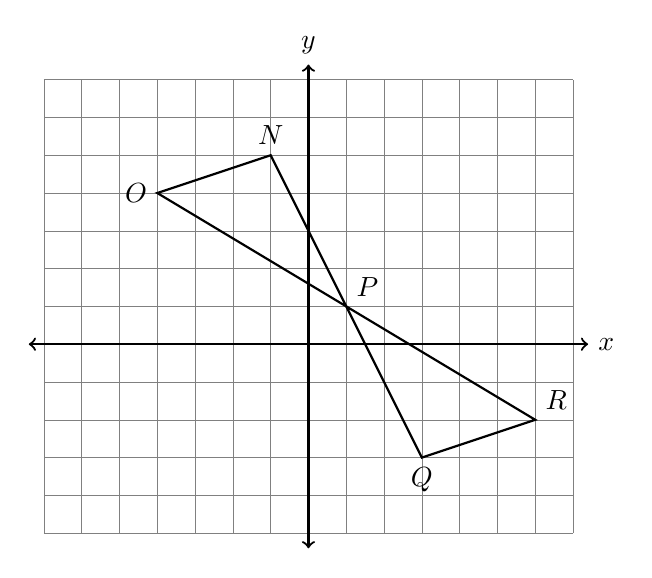
\begin{tikzpicture}[scale=.48]
        \draw [help lines] (-7,-5) grid (7,7);
        \draw [thick, <->] (-7.4,0) -- (7.4,0) node [right] {$x$};
        \draw [thick, <->] (0,-5.4)--(0,7.4) node [above] {$y$};  
        \draw [thick]
          (-1,5) node[above] {$N$}--
          (-4,4) node[left] {$O$}--
          (1,1) --cycle;
        \draw [thick]
        (3,-3) node[below] {$Q$}--
        (6,-2) node[above right] {$R$}--
        (1,1) node[above right] {$P$}--cycle;
      \end{tikzpicture}
    \end{flushright}

  
\end{enumerate}
\end{document}

